\documentclass{jarticle}
\usepackage{SICE-CCS}
\usepackage[dvipdfmx]{graphicx}
\usepackage{subfigure}
\usepackage{amsmath}
\usepackage{amssymb}
\usepackage{stmaryrd}
\usepackage{amsfonts}
\usepackage{bm}
\usepackage{ccaption}
\usepackage{comment}

\usepackage{multirow}
\pagestyle{empty}

\begin{document}

\title{ちびチャレ2019成果報告}
\author{B班(深津蓮,島田航太,吉内航,土屋一朗)}
\date{2019年4月26日}
\maketitle

\section{緒言}
近年,自動運転車を中心とした自律移動ロボットの研究開発が盛んに行われている.これらのロボットが自律移動を行うためには,自己位置推定,大域経路計画,局所経路計画,環境認識などが非常に重要である.これらの技術はROSのnavigation stack\cite{ns}などのオープンソースソフトウェアを用いて容易に実装可能である.しかし,今回はオープンソースソフトウェアを使用せずにそれらの技術を実装することで,コーティング技術と共に基礎的なロボット技術を学ぶことを目的とする.ハードウェアとしては,Roomba\cite{roomba}と2D-LiDARのUTM-30LX\cite{lrf},Raspberry PI Model B+\cite{raspi},C270 HD WEBCAM\cite{webcam},ノートPCを用いる.今回は,障害物を避け,白線を検知したら一回転し,最終的に明治大学生田キャンパス第二校舎D館1階を1周することを課題とする.
\section{提案手法}
本章では,提案システムにおける自己位置推定,大域経路計画,局所経路計画,白線検知について述べる.自己位置推定及び大域経路計画で用いる地図については,オープンソースソフトウェアのgmapping\cite{gmapping}を用いて作成した.システム図をFig.\ref{fig:system}に示す.

\subsection{自己位置推定}
自己位置推定にはAugmented Monte Carlo Localization(AMCL)\cite{localization}を用いた.観測モデルのノイズとして,正しい計測時の局所的な計測ノイズ,事前地図の中に存在しない物体による計測ノイズ,レーザがガラスなどを透過したことによる計測ノイズ,ランダムに発生する計測ノイズの4種類の観測ノイズを想定した.これらを導入することで,本試験中に想定されるノイズに対して強い尤度計算ができるようにした.また,Eq.\ref{eq:localization}に示す全パーティクルの平均に比例する確率$p$でランダムパーティクルを追加し,位置推定誤差からの復帰ができるようにした.ここで,$\omega_{fast}$,$\omega_{slow}$はそれぞれ尤度の短期および長期の平均値である.これと併用してパーティクルのxy座標およびyaw角の分散が閾値以下になると,最新の推定位置の周りにパーティクルを初期化することにより,システムのロバスト性を高めた.
\vspace{-3mm}
\begin{equation}
	p = max(0.0 , 1-\frac{\omega_{fast}}{\omega_{slow}})
\label{eq:localization}
\end{equation}
\begin{figure}
	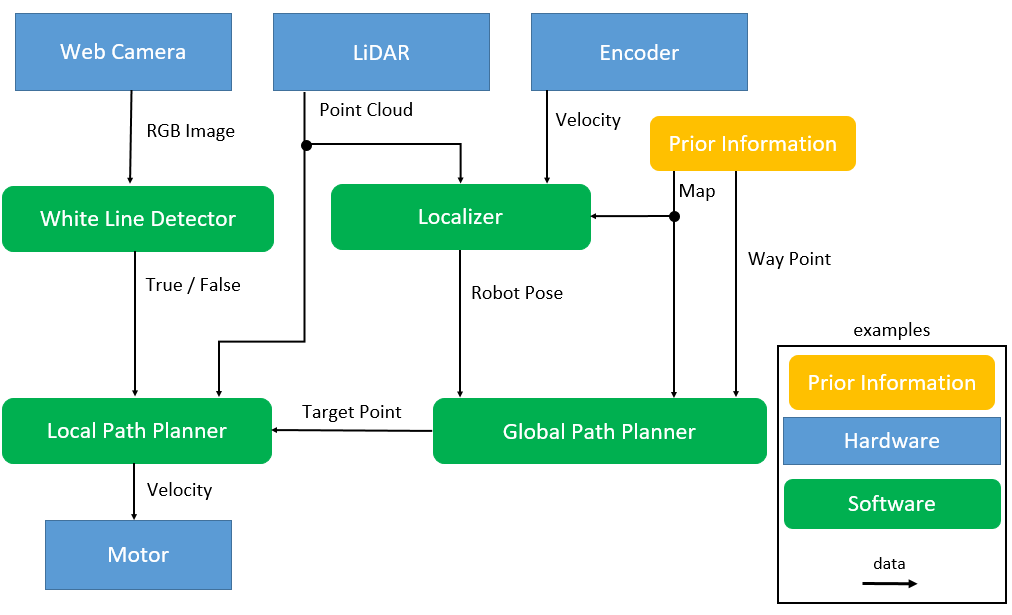
\includegraphics[width=7.5cm]{./picture/system.png}
	\caption{システム図}
	\label{fig:system}
\end{figure}
\begin{figure}
	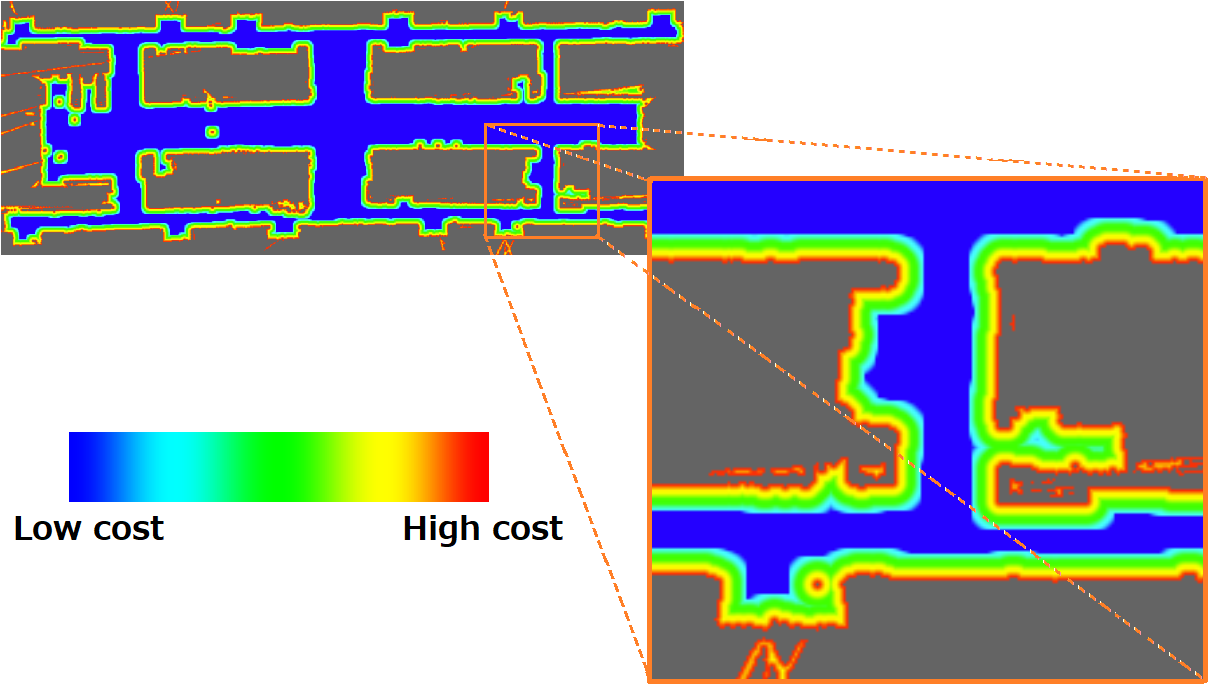
\includegraphics[width=7.5cm]{./picture/wallcostmap.png}
	\caption{w値のヒートマップ}
	\label{fig:wallcostmap}
\end{figure}
\vspace{-3mm}
\subsection{大域経路計画}
大域経路計画には,A*アルゴリズムを用いた.この経路計画において,地図はセルの集合として扱う.開始地点のセルから経路探索を始め,そのセルに到達するための最小コスト$g$と目標地点からの距離のヒューリスティック値$h$の和が最小のセルを選択して探索を進めていく.これにより,全経路を探索することなく最短経路を導き出すことができる.しかし,このままでは経路が壁に沿って壁と接してしまう.これを改善するために,h値とg値に壁からの距離に基づくw値を足した値をfとすることで壁から少し離れた経路を選択するようにした.Fig.\ref{fig:wallcostmap}にw値の地図上での分布を示す.また,最終的なfの値はEq.\ref{eq:globalpath}のようになる.
\vspace{-3mm}
\begin{equation}
	f = g + h + w
	\label{eq:globalpath}
\end{equation}
\subsection{局所経路計画} 
局所経路計画にはDynamic Window Approachを用いる.Dynamic Window内の速度$v$, 角速度$\omega$ をサンプリングし経路を予測する.Eq.\ref{eq:dwa}に示す評価関数を用いてコストを計算し,コストが最少となる速度$v$,角速度$\omega$を出力値とする.
\vspace{-3mm}
\begin{equation}
	\begin{split}
		G(v, \omega) &= \alpha obs(v, \omega) + \beta dis(v, \omega)\\
		&\quad+ \gamma heading(v, \omega) + \delta vel(v, \omega) 
	    \label{eq:dwa}
	\end{split}
\end{equation}
\vspace{-3mm}
ここで,評価関数には予測経路と障害物までの最短距離である$obs(v,\omega)$,最終予測位置から目標地点までの距離である$dis(v,\omega)$,目標位置に対する機体の向きである$heading(v,\omega)$,最高速度との差である$vel(v, \omega)$を用いる.特に,ゴールへの評価は距離と向きの二つを用いる.$α,β,γ,δ$は係数である.Fig.\ref{fig:DWA}に局所経路計画の評価のイメージを示す.
\begin{figure}
	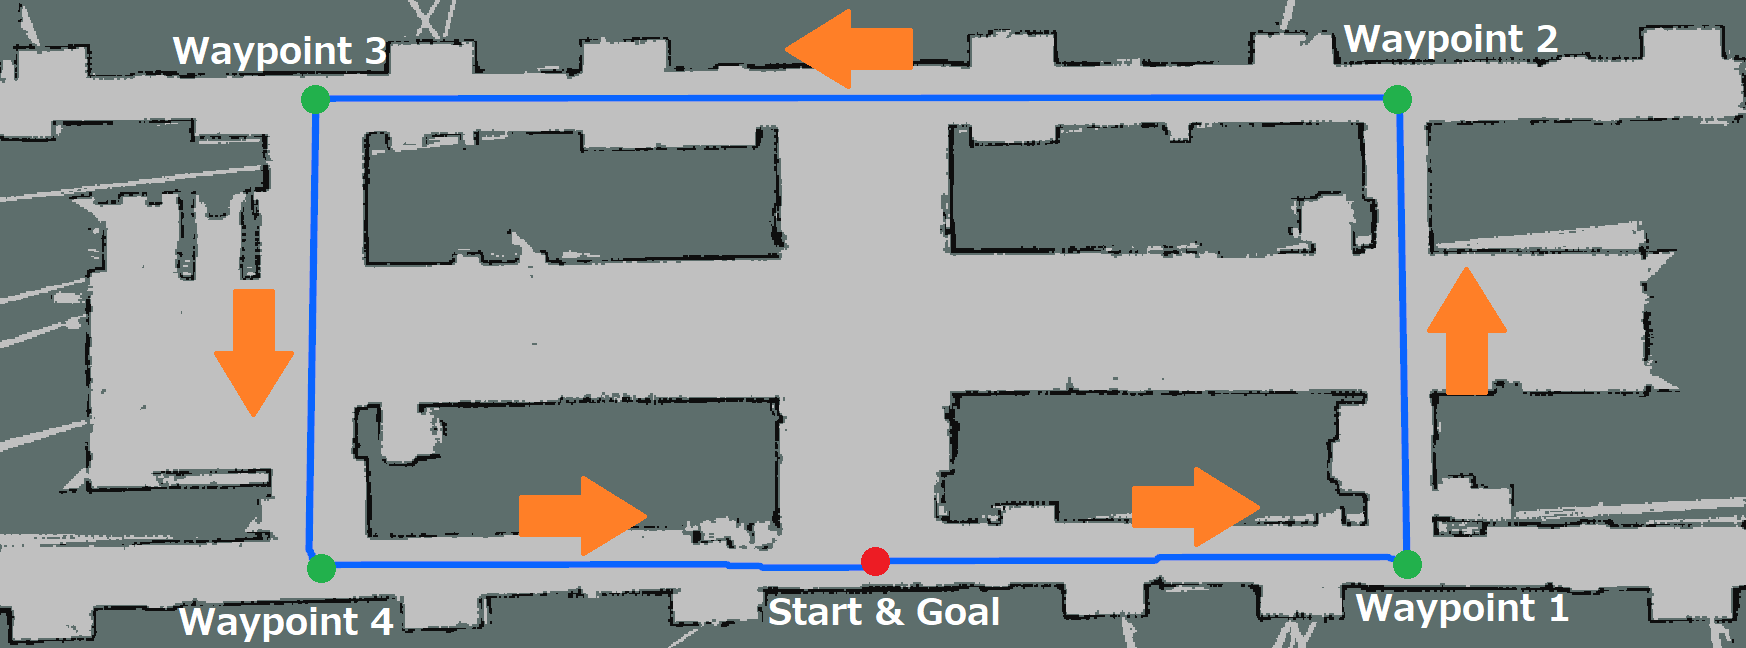
\includegraphics[width=8.5cm]{./picture/global_path.png}
	\caption{大域経路}
	\label{fig:globalpath}
\end{figure}

\begin{figure}
	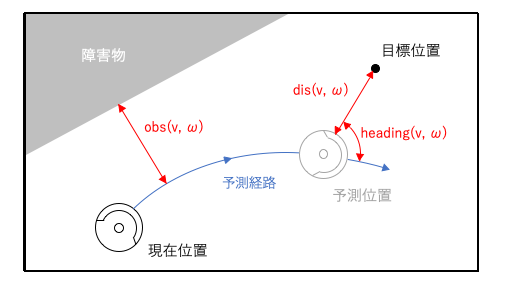
\includegraphics[width=8.5cm]{./picture/DWA.png}
	\caption{局所経路計画における評価}
	\label{fig:DWA}
\end{figure}

\subsection{白線検知}
白線検知にはオープンソースソフトウェアのOpenCV\cite{opencv}を用いて作成した.WEBCAMから取得したRBG画像を,グレー化,ぼかし,二値化,境界線の取得,面積によるフィルタリング,形状判断を行い,白線を検出した.以下に詳しく記述する.まず,WEBCAMからRBG画像を取得し,Eq.\ref{eq:gray}を用いてグレースケール画像を作成した.
\begin{equation}
	gray = Red * 0.299 +  Green * 0.587 + Blue * 0.114
	\label{eq:gray}
\end{equation}
そのグレースケール画像に対してガウシアンフィルタをかけ,二値化の際に画像が煩雑にならないようにした.また二値化では白線のみに反応するように,160を閾値として二値化した.今回の手法では黒い背景に白い物体がある想定で物体の輪郭を検出した.その後,その物体の輪郭から画像上の面積を取得して,大きすぎるものと小さすぎるものは除く処理を行った.また,画像の上半分は白線があると想定される床以外移すことが多いため,上半分にある輪郭は除く処理を行った.最後に,取得した輪郭を矩形で囲み,輪郭の面積$S_{contours}$と矩形の面積$S_{rectangle}$がEq.\ref{eq:kukei}を満たすものだけに絞ることで四角形の判断を行い,白線を検出した.
\begin{equation}
	S_{contours} > S_{rectangle} * 0.8
	\label{eq:kukei}
\end{equation}
\section{実験}
今回実装した自己位置推定,大域経路計画,局所経路計画、白線検知の評価のために,以下の実験を行った.
\subsection{周回実験}
本実験では,明治大学生田キャンパスのD館1階を一周させる実験を10回行う.Fig.\ref{fig:globalpath}にスタート地点・ゴール地点及び経由点を4点与えた時の1周の大域経路(青色)を示す.実験を行った結果,10回とも完走することができた.1周の平均走行時間は6分6秒だった.自己位置推定は,開けた場所に行った時や事前地図にない障害物を検知した時に多少の誤差が発生したが,短時間で復帰できることが確認できた.また,局所経路計画では,大域経路を沿うようにして走行し,壁や障害物に近づいた場合は避けることが確認できた.

\begin{figure}
	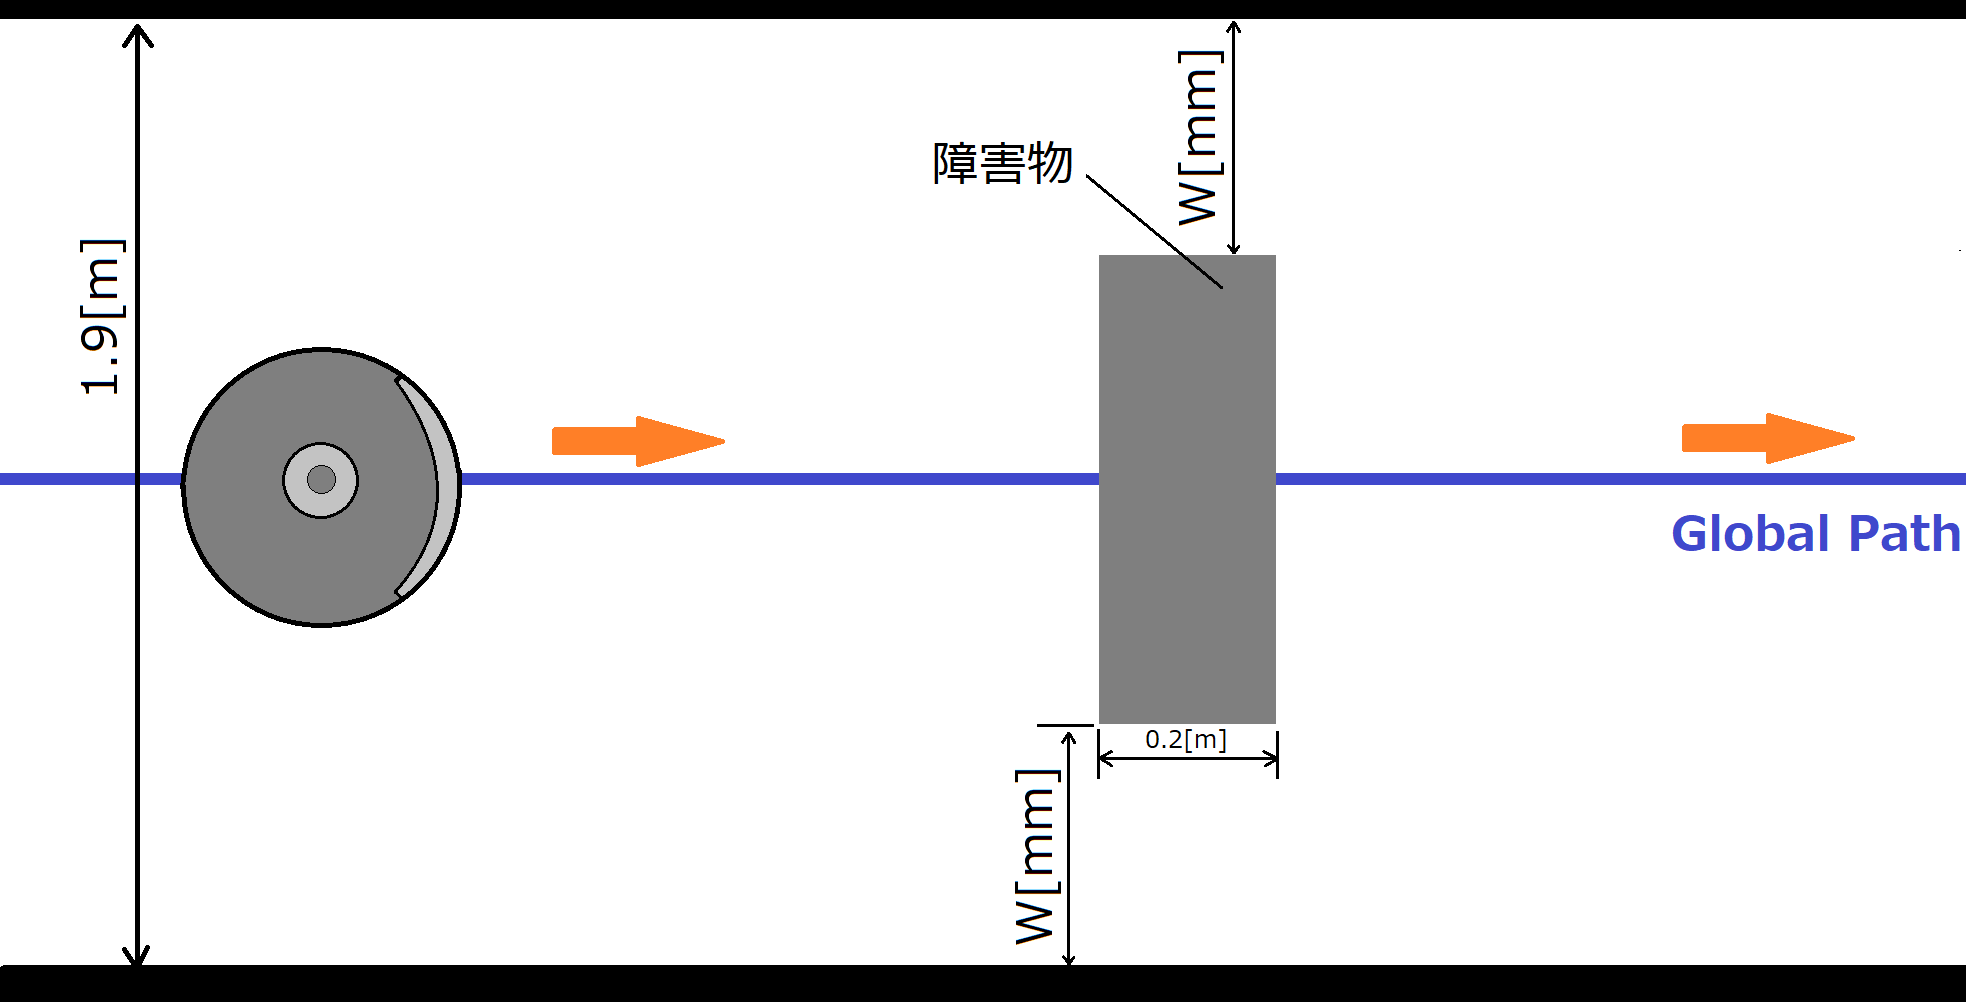
\includegraphics[width=7.5cm]{./picture/obstacle_test.png}
	\caption{障害物回避実験}
	\label{fig:obstacle_test}
\end{figure}

\subsection{障害物回避実験}
本実験では,障害物の回避性能を評価するため,Fig.\ref{fig:obstacle_test}に示すような回避実験を行った.$W$は障害物と壁の間の幅である.$W=0.6,0.7,0.8[m]$とし,各条件で回避し通過可能かどうかをそれぞれ5回走行させて調べる.実験の結果をTable.\ref{table:obstacle_test}に示す.壁と障害物の隙間が$0.7m$以下であると回避して通過する割合が下がり,$0.6m$以下になると通過することが全くできなかった.通過できなかった時は,壁の前でその場で回転し続けるという挙動を示した.これは目標地点に近づきかつ障害物を避ける経路が探索できなかったためと考えられる.
\begin{table}[h]
\caption{障害物回避実験結果}
\label{table:obstacle_test}
\begin{tabular}{|c|c|c|c|}
	\hline
	壁と障害物の距離W{[}m{]} & 0.8   & 0.7  & 0.6  \\
	\hline
	回避成功の割合          & 100\% & 80\% & 20\% \\
	\hline
\end{tabular}
\end{table}

\subsection{白線認識実験}
本実験では,周回実験の経路上に$50[cm]$の長さの白線を配置し,走行中に白線が検知できるかを確認した.白線を検知した場合5秒間停止するようにした.白線は各Waypoint4点とその間の3点の計7点に配置した。この実験結果をTable.2に示す.Waypoint間の白線検知は平均93\%の割合で検知し,Waypoint上の白線は平均65\%の割合で検知した.検知できなかった原因は機体が経路上からそれてしまい,カメラに白線の一部しか映らなかったことであり、カメラに白線の大部分が写っていた場合は検知することが確認できた.

\begin{table}[h]
\caption{白線検知実験結果}
\label{table:white_ditect}
\scalebox{0.8}{
\begin{tabular}{|c|c|c|c|c|c|}
\hline
             & 1回目   & 2回目   & 3回目  & 4回目   & 5回目   \\ \hline
Waypoint上の白線 & 75\%  & 25\%  & 75\% & 50\%  & 100\% \\ \hline
Waypoint間の白線 & 100\% & 100\% & 66\% & 100\% & 100\% \\ \hline
\end{tabular}
}
\end{table}

\section{結言}
本研修ではRoombaに2D-LiDARとカメラを搭載し,自律移動プログラムを実装した.実際に走行実験を行うことで,システムが有用であることを確認できた.本研修を通じて自律移動ロボットの基礎となる知識と技術を身につけることができ,gitを用いたチームでの開発の経験を積むことができた。これらは今後の研究を行っていくための基礎的な力となった。
\begin{thebibliography}{99}\scriptsize
	\bibitem{ns} http://wiki.ros.org/navigation
\vspace{-2mm}
	\bibitem{roomba} https://www.irobot-jp.com
\vspace{-2mm}
	\bibitem{lrf} https://www.hokuyo-aut.co.jp/search/single.php?serial=21
\vspace{-2mm}
	\bibitem{raspi} https://www.raspberrypi.org/products/raspberry-pi-3-model-b-plus/
\vspace{-2mm}
	\bibitem{webcam} https://www.logicool.co.jp/ja-jp/product/hd-webcam-c270
\vspace{-2mm}
	\bibitem{localization} Sebastian Thrun , Wolfram Burgard , and Dieter Fox 著,上田隆	一 訳,確率ロボティクス, 2007
\vspace{-2mm}
	\bibitem{opencv} https://opencv.org
\end{thebibliography}

\end{document}
